
\chapter{Adaptive remeshing}\label{chap:Adaptivity}

\section{Motivation}
Historically, numerical analysts concerned themselves
with \emph{a priori} error bounds of particular numerical
schemes, i.e.\@ \ asymptotic analyses of the order of convergence
of a discretisation with respect to some discretisation parameter
such as mesh sizing $h$ or polynomial order $p$. However, such
\emph{a priori} error bounds do not provide useful estimates
of the simulation error of a particular physical system on
a particular mesh for a specified norm: they merely describe
how that error behaves as the discretisation is modified. Since
such \emph{a priori} error bounds involve the unknown exact solution,
they are, in general, not computable.

In the late 1970s, the pioneering work of Babu\v ska
and Rheinboldt laid the foundations for \emph{a posteriori}
error estimates \citep{babuska1978,babuska1978b}.
In contrast to \emph{a priori} bounds,
\emph{a posteriori} error estimates involve only
the approximate computed solution and data from the problem,
and are thus computable (or approximately so, if they involve the
solution of an auxiliary problem). These error
estimates can then be used in an adaptive loop, modifying
the discretisation until some user-specified error criterion
is reached. Most \emph{a posteriori} error estimation literature deals with estimating
the error in the natural norm induced by the bilinear form
of the problem, the energy norm.
For a review of \emph{a posteriori} error estimation
with emphasis on energy norm estimation
see the books of Verf\"urth \citep{verfurth1996} and
Ainsworth and Oden \citep{ainsworth2000}. The goal-oriented
adaptive framework of Rannacher and co-workers, which estimates
the error in the computation of a given goal functional, is detailed
in \citet{becker2001} and \citet{bangerth2003}.

Once \emph{a posteriori} estimates have been computed,
there are many possible ways of modifying the discretisation
to achieve some error target. These include $h$-adaptivity,
which changes the connectivity of the mesh \citep{berger1989}; $p$-adaptivity,
which increases the polynomial order of the approximation
\citep{babuska1994}; and $r$-adaptivity, which relocates
the vertices of the mesh while retaining the same connectivity
\citep{budd2009}. Combinations of these methods are also
possible (e.g., \citet{houston2001,ledger2003}).

This review focuses on adaptive remeshing in multiple dimensions, as this is
the technology available in \fluidity.
This approach is the most powerful of all $hr$-adaptive methods, since the meshes produced are not constrained
by the previous mesh; therefore, this approach allows for maximum flexibility in
adapting to solution features. However, this flexibility comes
at a cost: guiding the adaptive remeshing procedure (choosing
what mesh to construct), executing the adaptation (constructing
the chosen mesh) and data transfer of solution fields (from the previous mesh to
the newly adapted mesh) become more complicated than with hierarchical refinement.

This chapter is divided as follows. Firstly, we orient the user by describing a typical
adaptive loop used in \fluidity\ (section \ref{sec:typical_adaptive_loop}). Before
discussing how to configure mesh adaptivity, we introduce some necessary background ideas: 
section \ref{sec:meshes_and_metrics} describes how a metric tensor field
may be used to encode the desired mesh, and section \ref{sec:adaptive_remeshing_technology} describes how the
mesh optimisation procedure in \fluidity\ uses this metric tensor to generate an adapted mesh. Finally,
the chapter ends with a discussion of how to use mesh adaptivity in \fluidity, with a discussion
of the various algorithms offered and their advantages and disadvantages (section \ref{sec:using_mesh_adaptivity}).

\section{A typical adaptive loop} \label{sec:typical_adaptive_loop}
This section presents a typical adaptive loop, as used in the lock--exchange example, section \ref{sec:lock_exchange}
(examples/lock\_exchange/lock\_exchange.flml).

\begin{enumerate}
\item The initial conditions of the prognostic variables (velocity, temperature) are applied.
\item The adaptive procedure is invoked 6 times to adapt the initial mesh to represent the
desired initial conditions. This involves:
  \begin{enumerate}
  \item Computing the Hessian of velocity (which is zero, as the initial velocity condition is zero).
  \item Converting the Hessian of velocity into a metric tensor (in this case, the tensor will request the maximum
        edge length size everywhere, as velocity can be represented exactly). This depends on the norm chosen and the minimum
        and maximum edge length sizes.
  \item Computing the Hessian of temperature (which is nonzero, as the initial temperature condition is a step-function).
  \item Converting the Hessian of temperature into a metric tensor (in this case, the tensor will request fine resolution
        at the step, and the maximum edge length size everywhere else).
  \item The size requirements of these two metrics are merged to give one metric tensor describing the desired mesh.
  \item The metric is then smoothed with a gradation algorithm to avoid large jumps in mesh sizing.
  \item The metric is scaled so that the expected number of nodes it will yield after adapting is no more than the maximum number of nodes.
  \item The metric is then passed to the adaptivity algorithm, which modifies the mesh until it satisfies the sizing requirements given in the metric.
  \item Since the simulation time has not yet advanced, the initial conditions are reapplied on the newly-generated adapted mesh. 
  \end{enumerate}
     This procedure is iterated 6 times so that the adaptive algorithm can recognise the anisotropy of the step.
\item Once the initial mesh has converged, the simulation time loop proceeds. The lock--exchange simulation invokes
the adaptive algorithm every 10 timesteps to ensure that the dynamics do not extend beyond the zone of adapted
resolution. Each invocation of the adaptive algorithm involves:
  \begin{enumerate}
  \item Computing the Hessians of velocity and temperature (both of which will be nonzero).
  \item Converting the Hessians to metrics (again depending on the norms chosen and the minimum and maximum edge length sizes).
  \item Merging the metrics for each field to yield a combined metric which satisfies both of their size demands.
  \item The metric is then smoothed and scaled, as before, and passed to the adaptivity library.
  \item Once the adaptivity library is finished, the field data from the previous mesh is transferred to the new mesh by interpolation.
  \end{enumerate}
\end{enumerate}

\section{Representing meshes as metric tensors} \label{sec:meshes_and_metrics}
The process of adaptive remeshing divides naturally into three parts. The first is to
decide what mesh is desired; the second is to actually generate that mesh; the third is to
transfer data from the old mesh to the new mesh. The form
of communication between the first two stages is a \emph{metric}: a symmetric positive-definite tensor field
which encodes the desired geometric properties of the mesh. This representation was first introduced
in \citet{vallet1990}, and has proven key to the success of adaptive remeshing methods.
This section describes the mathematical details of how a metric encodes the desired size
and shape information: however, understanding this section is not necessary to successfully
use adaptivity in \fluidity.

Firstly, consider how the size and shape information about a mesh might be encoded. A natural
first attempt would be to define a size function $h(x)$ which describes the desired mesh
spacing at a particular point. This works, and is used in many isotropic adaptive algorithms.
However, its deficiency becomes clear when we consider the anisotropic examples that we
wish to exploit: consider again the step function initial condition of the lock--exchange
example. In this case, we want the mesh sizing across the step to be small (to capture the
jump), but we want the mesh sizing along the step to be large (parallel to the step, the
field does not change at all). Therefore, the \emph{mesh sizing desired is not only a function
of space, it is also a function of direction}. At a given point, the desired mesh sizing differs
in different directions. This cannot be encoded in a scalar size function, as that associates
only one number with each point in space. The solution to this problem is to increase the rank
of the object returned by the size function, from a rank-0 single real value to a rank-2 tensor.

Let $M$ be a symmetric positive-definite tensor (constant over the domain for now).
$M$ induces an inner product by
\begin{equation}
\langle x, y\rangle_M = x^T M y
\end{equation}
and so $M$ also induces a notion of distance between two points in the usual manner:
\begin{equation}
d_M(x, y) = ||x - y||_M = \sqrt{\langle x - y, x - y \rangle}.
\end{equation}
Note that the symmetric positive-definite condition is necessary for the tensor
to induce a sense of distance: for otherwise, the tensor does not induce
a norm. 

Now let $\metric$ be a symmetric positive-definite tensor field. As long as
$\metric$ is sufficiently smooth, then it also induces an inner product
(see \citet{simpson1994} for details). We say that a mesh $\cal{T}$ satisfies
$\metric$ if every edge has unit edge length with respect to its inner product;
$\cal{T}$ is a unit mesh with respect to this metric.

The metric \emph{warps space}, in the same manner that space is warped in General Relativity.
The metric encodes a new sense of distance, and a regular unit mesh (a mesh of edge length
one) is built with respect to this new sense of distance. For example, if the metric encodes
that two points are ``far apart'', then when a unit mesh is built, many mesh
nodes will lie between them, and the mesh concentration will be dense. Conversely, if the metric
encodes that two points are ``close together'', then when a unit mesh is built,
few mesh nodes will lie between them and the mesh concentration will be sparse.

In the adaptive procedure employed in \fluidity, the metric passed to the adaptivity
library encodes the desired mesh sizing. That is, the adaptive procedure is a function
that takes in a metric and returns a mesh matching that metric. Conversely, it is also
possible to derive the metric for a given mesh. In order to see how the metric representing a mesh may be derived, consider the transformation from the reference element to the physical
element inherent in the finite element assembly procedure \citep{femtools}.
Let $K$ be an element of a linear simplicial mesh. $K$ is geometrically characterised by the affine map
$T_K: \hat{K} \rightarrow K$, where $\hat{K}$ is the reference isotropic element. Since
$T_K$ is assumed affine, we can write this transformation as
\begin{equation}
x = T_K(\hat{x}) = J_K\hat{x} + t_K,
\end{equation}
where $J_K$ is the Jacobian of the transformation. The metric for this element is derived
from the polar decomposition of the Jacobian, which yields
\begin{equation}
J_K = M_K Z_K
\end{equation}
where $M_K$ is a symmetric positive-definite matrix referred to as the metric,
and $Z_K$ is orthogonal \citep{micheletti2006}. The geometric properties of a simplicial mesh can be represented
as a piecewise constant (\Pzero) field over it. The same argument applies to
nonlinear or non-simplicial elements, but here the Jacobian varies over the element,
and so the metric does too.

The book of \citet{george1998} gives a thorough discussion of the role of metrics
in mesh adaptivity. F. Alauzet and co-workers have recently published some thought-provoking
papers advocating that metrics are in fact the continuous analogue of meshes: in the same
way as the continuous equations are discretised to yield the discrete equations, a continuous
metric is discretised to give a mesh on which those equations are solved. For more details, see
e.g. \citet{alauzet2006b,courty2006,alauzet2008,loseille2010i,loseille2010ii}.

\section{Adaptive remeshing technology} \label{sec:adaptive_remeshing_technology}
This section briefly reviews the second problem solved by the adaptivity algorithm: given the desired
size and shape information, how can a mesh satisfying this be generated?

Given a metric $\metric$, there are three main ways to generate a mesh which satisfies
that metric: global remeshing, local remeshing, and mesh optimisation. For a thorough discussion
of the history of these three approaches, see \citet{farrell2009i}.

Global remeshing is the act of generating an entirely new mesh of the same domain satisfying the sizing
specification, by means of an automatic mesh generator. This was first introduced in \citet{peraire1987} by incorporating
sizing and directionality inputs to an advancing front mesh generator. While this is the fastest
approach if the existing mesh and the desired mesh are very different, developing a robust metric-aware
mesh generator is very difficult, and to the best of the author's knowledge no open-source algorithm
is available for this problem. 

By contrast, local remeshing is a mechanism of adaptive remeshing in which cavities of elements are removed
and the hole remeshed \citep{hassan1998}. These cavities are identified by measuring
their conformity to the given sizing specification. Again, this relies on the availability of a robust
metric-aware mesh generator to fill the cavities.

Mesh optimisation is a mechanism of adaptive remeshing which deforms the previous mesh
to the adapted mesh by a sequence of local operations. The first ingredient in a mesh optimisation algorithm is the functional: how
the quality of an element is determined, and how one element is deemed better than
another. In the adaptive remeshing case, the functional is the point at which the metric
comes in to play: the basic job of the functional is to measure the compatibility of the
element to the metric specifying the size and shape of that element. Many different functionals
have been considered in the literature: for a review, see \citet{knupp2003}. For the
functional used in the 2D case, see \citet{vasilevskii1999}; for the functional used in the
3D case, see \citet{pain2001}.

The second ingredient in a mesh optimisation algorithm is the set of operations the
algorithm may perform in an attempt to improve the mesh. Example operations might include
merging adjacent elements, splitting an element into two or more child elements, swapping
edges or faces, and moving nodes in the mesh. For diagrams of some example optimisation
operations see figure \ref{fig:edge_operations}.

\begin{figure}[h] 
\centering
\subfigure[2D]{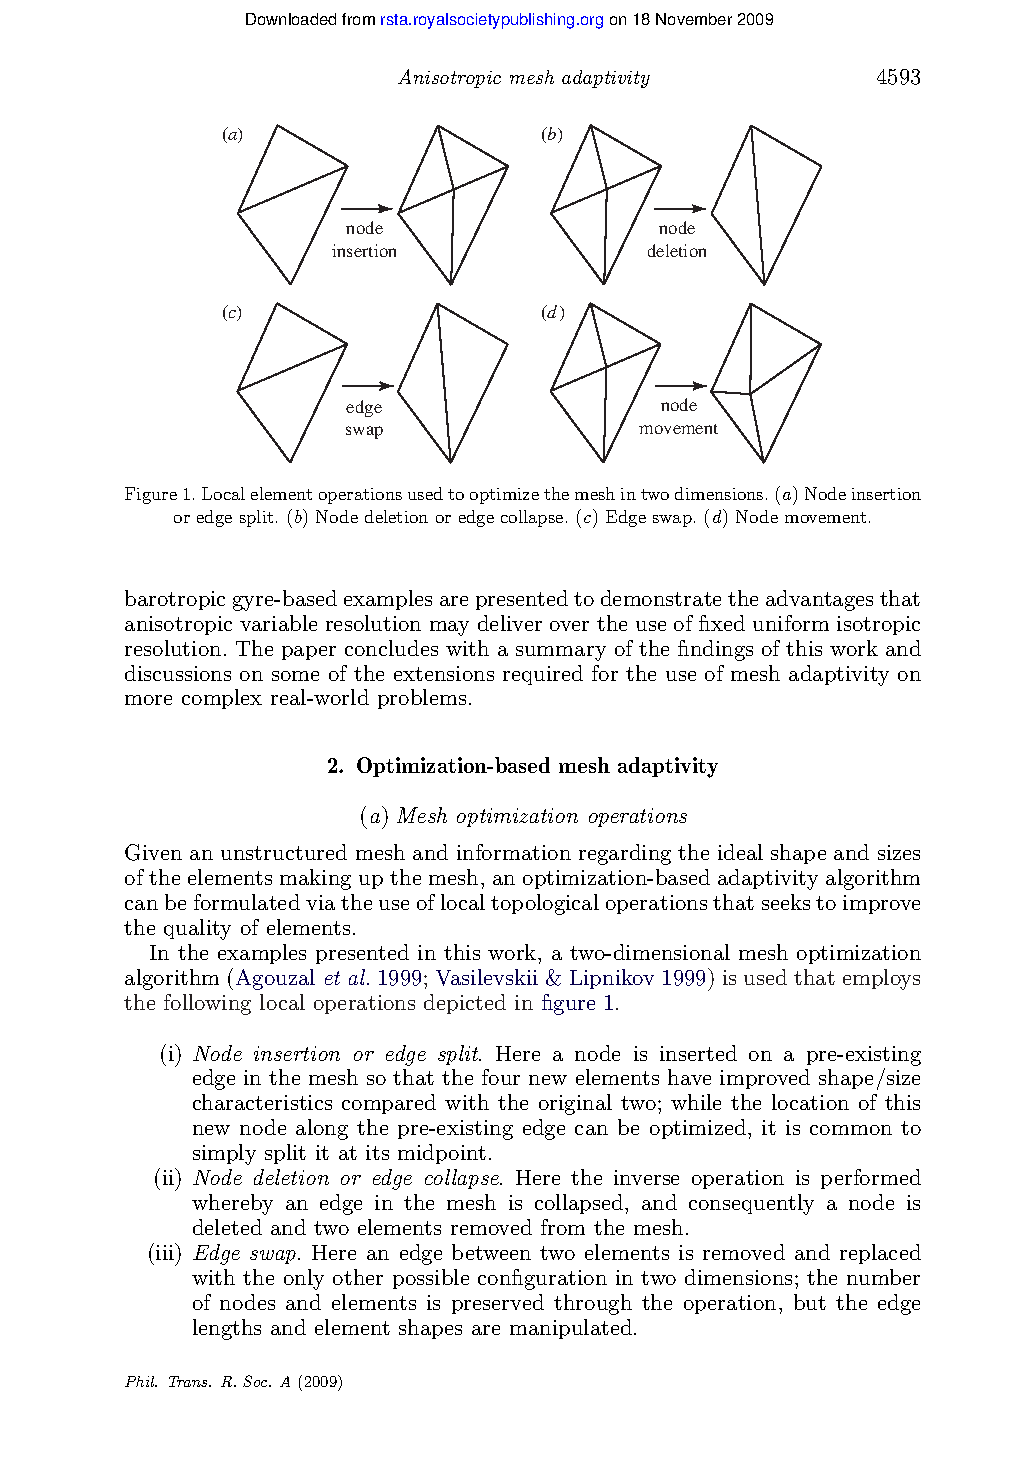
\includegraphics[width=0.475\textwidth, clip = True, trim = 35mm 165mm 32.5mm 20mm]{./adaptivity_images/piggott2009_pg4}} \hspace{7mm}
\subfigure[3D]{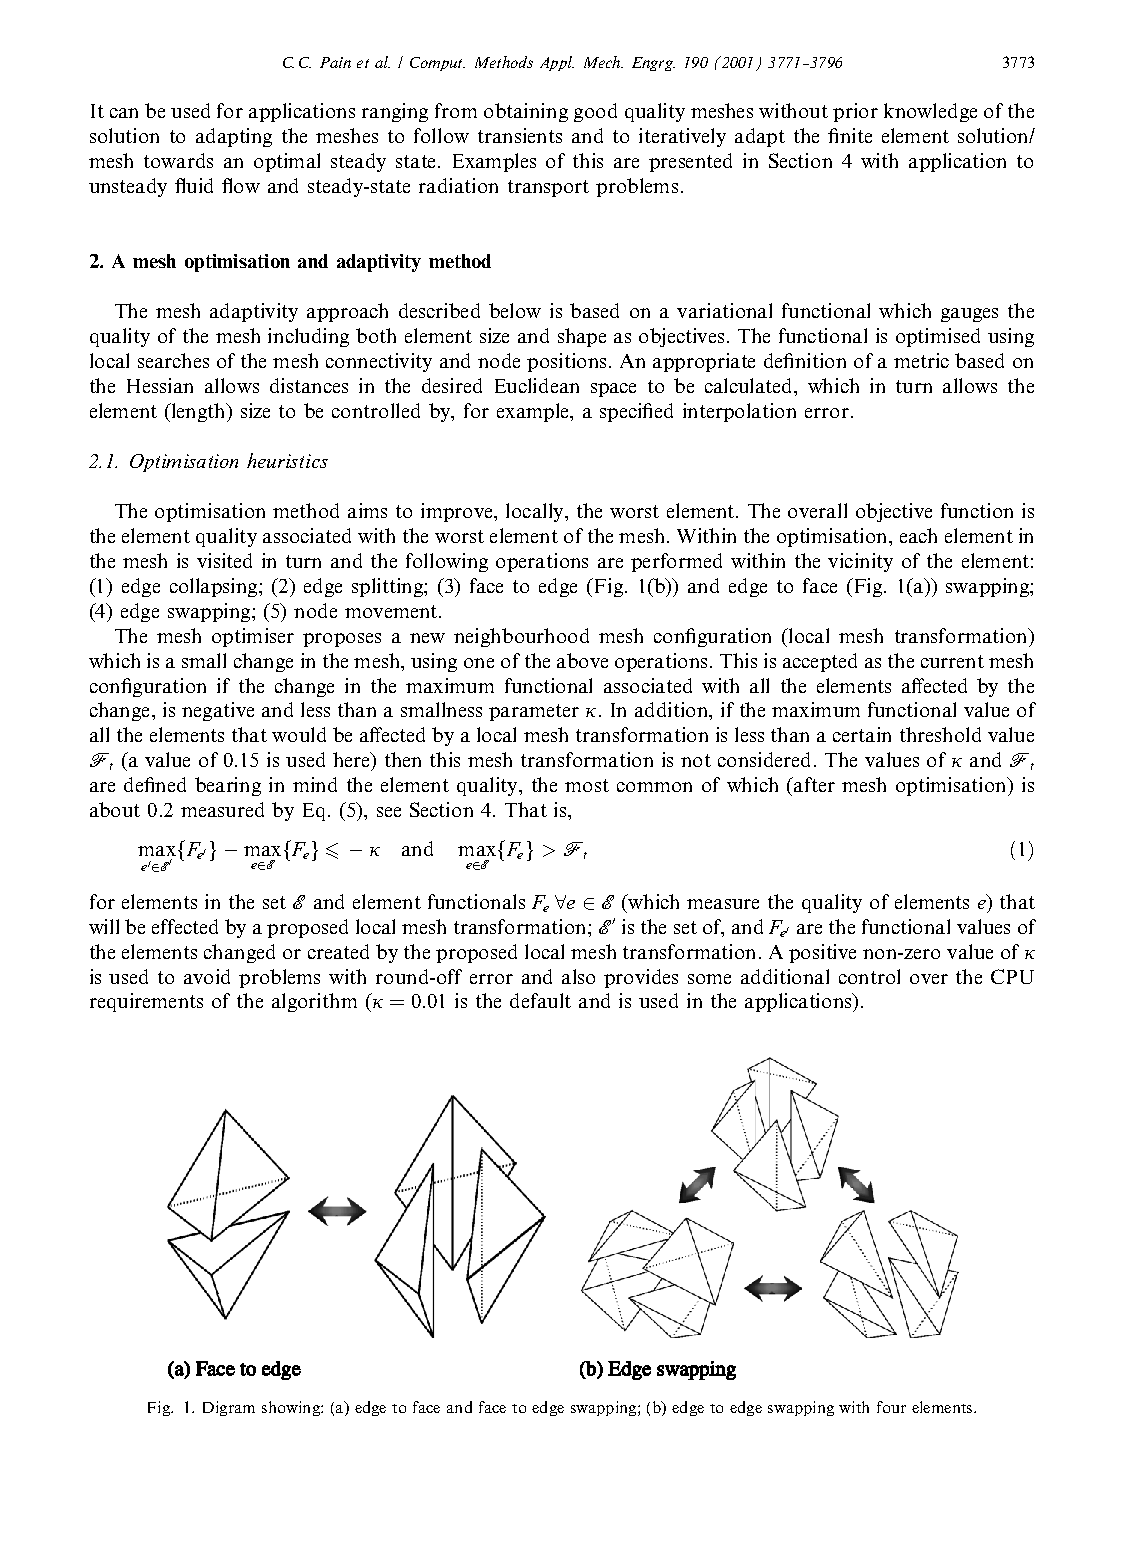
\includegraphics[width=0.45\textwidth, clip = True, trim = 25mm 35mm 95mm 185mm]{./adaptivity_images/pain2001_pg3}}
\caption[Example of mesh modification operations.]{Example of mesh modification operations. (a): Node insertion or edge splitting, node deletion or edge collapse, edge swap and node movement in two dimensions \citep[2D, from][]{piggott2009}. (b): Edge to face and face to edge swapping in three dimensions \citep[3D, from][]{pain2001}.}
\label{fig:edge_operations}
\end{figure}

The mesh optimisation library provisionally executes one or more optimisation operations, and then
invokes the functional to decide whether those operations improved the mesh. If the
mesh was improved, then the proposed changes are committed; otherwise, they are reverted. The
scheduling of the operations has a large impact on the effectiveness of the procedure \citep{li2005},
and ensuring that the optimisation operations are robust is quite delicate \citep{compere2010a}.

Mesh optimisation is available by default in three dimensions using the algorithm
of \citet{pain2001}. It is available in two dimensions using the \texttt{mba2d} algorithm of
\citet{vasilevskii1999} if \fluidity\ was configured with
the \configureflag{--enable-2d-adaptivity} flag, section \ref{sec:configuring_the_build_process}; this is not enabled by default
as \texttt{mba2d} is licensed under the GPL, while \fluidity\ is licensed under the LGPL,
and so its default inclusion would cause licensing complications.

\section{Using mesh adaptivity} \label{sec:using_mesh_adaptivity}
This section contains the practical advice for configuring and optimising
adaptive simulations. Further information about the configuration options can be found in section \ref{sec:config_adapt}

The first golden rule is to start with a fixed-mesh simulation that works
(i.e., gives sensible answers for the resolution used). Mesh adaptivity is a complex
extra nonlinear operation bolted on to the discretisation, and it will make reasoning
about and debugging the simulation more difficult. Therefore, make sure that you
are happy with the well-posedness of the problem, the stability of the discretisation,
the convergence of the solutions, etc. before attempting to employ adaptivity.

Secondly, be aware that employing adaptivity can require a nontrivial amount of tuning
to get exactly the result desired. Be prepared to iterate on the adaptivity settings,
and make changes conservatively, one parameter at a time. As you gain more experience
of the adaptivity options offered in \fluidity, it will become easier to identify
problems and how they can be solved.

As a first step, configure \fluidity\ to adapt only to one field, usually the most
important in the simulation. The adaptivity options for each field are found in the
\option{\ldots/adaptivity\_options} option under each field. As the initial settings,
choose \option{absolute\_measure} (section \ref{sec:absolute_metrics}), and set \option{p\_norm}
to 2 (section \ref{sec:norm_choice}). This configures the metric to optimise for the $L_2$ norm
of interpolation error. Under the \option{InterpolationErrorBound}, set the value to a constant,
and as an initial guess use 10\% of the $L_2$ norm of the field under consideration (this
value is available in the .stat file). See section \ref{sec:adaptivity_weights} for more information
about this setting. Unless you are running a simulation with DG fields, leave the interpolation
algorithm as \option{consistent\_interpolation}; if you have DG fields, set their interpolation
algorithm to \option{galerkin\_projection}. This is explained in further detail in section \ref{sec:interpolation_algorithms}.

Field-specific adaptivity options are configured under the field in question, and non-field-
specific options are configured in \option{/mesh\_adaptivity/hr\_adaptivity}. It is recommended
that the operator first configure the adaptivity options so that it is only invoked at the
very start of the simulation (using the \option{adapt\_at\_first\_timestep} option), and only once this is configured satisfactorily move on to dynamic adaptivity. There are several reasons for this. Firstly, since the adaptive algorithm is invoked
at the start of the simulation, the time between configuration and feedback is lessened, making it
easier for the operator to get a feel for the effect of the different settings. Secondly, since the
system state at the initial condition is known exactly, the complicating effects of interpolation
algorithms are excised. Thirdly, accurately representing the initial condition is usually a requirement
for a sensible answer at later simulation times, and so configuring the initial adaptivity is
necessary anyhow.

For the initial adaptive configuration, set the period in timesteps to 20, and the maximum number
of nodes to be 200000 times the number of processors you are using. (This is deliberately set high
so that it does not influence the mesh produced; later on, it can be turned down to control the
computational requirements of the simulation. See section \ref{sec:max_min_nodes}.) Under \option{/mesh\_adaptivity/hr\_adaptivity/enable\_gradation},
set the \option{gradation\_parameter} to 2. This allows the edge length to double from element to element,
and is quite a weak gradation parameter. (Again, we wish to minimise the influence of the gradation
algorithm on the mesh produced; if necessary, the metric can be smoothed by reducing this value. See section
\ref{sec:gradation_parameter}.) Under \option{/mesh\_adaptivity/hr\_adaptivity/tensor\_field::MaximumEdgeLengths/anisotropic\_symmetric/constant},
set the \emph{diagonal} entries to the diameter of your domain. (The maximum edge length can be anisotropic,
in the same way that the desired edge length can be anisotropic. See section \ref{sec:max_min_edge_length}.)
Similarly, under \option{\ldots/tensor\_field::MinimumEdgeLengths/anisotropic\_symmetric/constant}, set the
\emph{diagonal entries} to something small (e.g., the diameter of the domain divided by 10000). Again, we wish
to remove the influence of these settings by default, so that their effect can be applied by the operator
if it is desired.

Activate \option{/mesh\_adaptivity/hr\_adaptivity/adapt\_at\_first\_timestep}, and set the \option{number\_of\_adapts}
to 6. Under \option{/mesh\_adaptivity/hr\_adaptivity/debug}, activate the \option{write\_adapted\_state} option. This
ensures that after each invocation of the adaptivity algorithm the mesh is dumped, so that the convergence of
the adaptive algorithm for the initial condition may be inspected. Finally, configure the timestepping
options so that the simulation terminates after one timestep, so that the adaptivity settings may be configured
for the initial condition.

Now run the problem, and inspect the adapted\_state\_*.vtu that result. Each VTU is the \emph{output}
of the adaptivity loop, and hopefully convergence of the adaptive procedure towards some 
mesh should be observed. If the adapted mesh is satisfactory, then record the adaptivity parameters
used for this field, and repeat the procedure on any other fields to which you wish to adapt that
have nontrivial boundary conditions. Once you are happy with the initial mesh, run the simulation further
and inspect the output of the adaptivity library, tuning the parameters to get the optimal mesh. (In this case, you may wish to cache the output of
the adaptation to the initial condition with \option{/mesh\_adaptivity/hr\_adaptivity/adapt\_at\_first\_timestep/output\_adapted\_mesh}.)
The following sections offer guidance on the parameters that can be varied and the effect that
this has on the adaptive simulation.

\subsection{Choice of norm} \label{sec:norm_choice}
The basic strategy used to compute the error metric is to \emph{control the interpolation
error} of the function represented. Let $f(x)$ be a continuous, exact field, and let
$f_h(x)$ be its representation on the finite element mesh. Then, the interpolation error
is defined as $\left| f - f_h \right|$, which is itself a function over the domain $\Omega$.
The ``size'' of this interpolation error may be quantified in different ways, using different norms.
Historically, the interpolation error was first controlled in the $L_{\infty}$ norm, which considers
the maximum value of the interpolation error over the domain. The metric formulation which
controls the $L_{\infty}$ norm is the simplest, and remains the default in \fluidity. Since the $L_{\infty}$
norm considers only the least accurate point in the domain, without regard to the relative size of the
interpolation error there, then it can have a tendency to focus the resolution entirely on the 
dynamics of largest magnitude. Other authors have instead proposed the use of the $L_p$ norm, which incorporates
more influence from dynamics of smaller magnitude \citep{alauzet2008,loseille2010ii}. Empirical experience indicates that choosing $p=2$, and hence the $L_2$ norm, generally gives better results, and for that reason we recommend it as the default for all new adaptivity configurations.

\subsection{Absolute, relative and $p$-- metrics} \label{sec:absolute_metrics}
Consider again the metric for controlling the $L_{\infty}$ norm of the interpolation error. This metric takes the form
\begin{equation}
M = \frac{\left|H\right|}{\epsilon},
\end{equation}
where $H$ is the Hessian of the field under consideration and $\epsilon$ is the target interpolation error. As mentioned
in the previous section, this metric tends to neglect smaller-scale dynamics, and so \citet{castrodiaz1997} proposed
an alternative metric formulation to fix this. They suggested to compute
\begin{equation}
M = \frac{\left|H\right|}{\max(\epsilon \cdot \left|f\right|, \epsilon_{\textrm{min}})},
\end{equation}
where $f$ is the field under consideration, $\epsilon$ is now a \emph{relative tolerance}, and $\epsilon_{\textrm{min}}$ is a
user-configurable parameter. For example, if $\epsilon = 0.01$, then the tolerance on the denominator of the metric formulation
will be 1\% of the value of the field, and so it will scale the target interpolation error with the magnitude of the field.
$\epsilon_{\textrm{min}}$ is the minimum tolerance, and is employed to ensure that the denominator never becomes zero.
However, empirical experience indicates that this metric formulation is very sensitive to the value of $\epsilon_{\textrm{min}}$,
and that it generally yields poor results. The approach of using the $L_p$ norm instead of the relative $L_{\infty}$ norm is much more mathematically rigorous, and for this reason the relative metric option is deprecated.

The metric that controls the $L_p$ norm of the interpolation error takes the form \citep{chen2007,loseille2010ii}
\begin{equation}
M = \det\left|H\right|^{-\frac{1}{2p+n}} \frac{\left|H\right|}{\epsilon} \, ,
\end{equation}
where $p \in \mathbb{Z}$ and $n$ is the dimension of the space.

The options for the metric are selected by field and can be found under \option{name\_of\_field/adaptivity\_options}. For more information see section \ref{sec:configuring_fluidity_error_metric}.

\subsection{Weights} \label{sec:adaptivity_weights}
The target value of the norm of the interpolation error is set in the \option{InterpolationErrorBound}
field under the \option{\ldots/adaptivity\_options} for a particular field. Usually, this
will be constant throughout space and time, but advanced users may wish to vary this, and so
it is possible to set this value as a Python field. When configuring an adaptive simulation
for the first time, the general advice would be to start with a high weight and thus a high
interpolation error ($10\%$ of the range of the field is a good rule of thumb), and reduce the weight as necessary to represent the desired dynamics.
In all cases, the field weights should be the main parameters to vary to control the resolution
of the adapted meshes.

\subsection{Gradation parameter} \label{sec:gradation_parameter}
In numerical simulations, a smooth transition from small elements to large elements is generally important for mesh quality. 
A mesh sizing function derived from error considerations may
yield sudden changes in desired mesh edge length, due to the
nature of the problem being resolved. Such sudden changes are undesirable
in a mesh:
for example, sudden changes in mesh sizing
can cause the spurious reflection of waves \citet{bazant1978,bangerth2001}.
Therefore, a mesh gradation algorithm
is applied to smooth out sudden variations in the mesh sizing function.

Various mesh gradation algorithms have been introduced to solve this problem.
\citet{lohner1996} uses various functions of distance to point sources where edge
length is specified by the user to control the isotropic sizing function for an
advancing front grid generator. \citet{owen2000} applies natural neighbour
interpolation to smooth sudden variations in an isotropic sizing function.
\citet{persson2006} bounds the gradient of an isotropic sizing function by
solving a partial differential equation. \citet{borouchaki1998} introduced two
gradation algorithms for scalar isotropic mesh sizing functions, bounding the
gradient of the sizing function or the ratio of the length of two adjacent
edges, along with anisotropic generalisations of these. These algorithms have
been successfully applied in many diverse application areas (e.g.
\citet{frey2004, alauzet2003, laug2002, lee2003}).

\fluidity\ uses an algorithm based on that of \citet{borouchaki1998}. It has only one
user-configurable parameter, \option{/mesh\_adaptivity/hr\_adaptivity/enable\_gradation/gradation\_parameter}.
This number constrains the rate of growth in desired edge lengths along an edge. A value
of 1 would force the mesh to have constant edge length everywhere. A value of 2 would allow
desired edge lengths to double from node to node. The default value is 1.5. Optionally, the
algorithm may be disabled by choosing \option{/mesh\_adaptivity/hr\_adaptivity/disable\_gradation}
instead of \option{/mesh\_adaptivity/hr\_adaptivity/enable\_gradation}.

\subsection{Maximum and minimum edge length tensors} \label{sec:max_min_edge_length}
For robustness of the mesh adaptivity procedure, and to limit refinement/coarsening of the
mesh it is possible to set maximum and minimum allowed edge length sizes. The input to
these quantities are tensors allowing one to impose different limits in different directions.
Assuming that these directions are aligned with the coordinate axes allows one to define
diagonal tensors.

There are both good and bad reasons that one may need to impose these constraints. The good
reasons are based on physics: a maximum size may be based on the size of the domain, or that it
resolves a spatial scale that allows an instability to develop (the latter case would be better
handled with a more advanced \emph{a posteriori} error measure of course), or simply a consequence of
the time/memory constraints of the machine the problem is running on. The bad reason is to control
the mesh when the field weights have been chosen poorly. However, it is often 
unavoidable that the weights and max/min edge length sizes will be chosen in tandem to achieve 
an appropriate mesh, especially for experienced users --- new users should be wary whenever maximum
and particularly minimum size constraints are actually hit in the mesh and as a first stage should
look to vary the weights to achieve the mesh they desire.

Finally, note that these constraints are achieved through manipulations to the metric, which in turn
controls an optimisation procedure. They are therefore not hard constraints and one may observe the
constraints being broken (slightly) in places.

\subsection{Maximum and minimum numbers of nodes} \label{sec:max_min_nodes}
Similar to the edge length size constraint above, it is possible to limit the maximum and minimum number of nodes
that the mesh optimisation procedure returns. For reasons very similar to above this is potentially dangerous, 
but somewhat necessary. 

This is effected by computing the expected number of nodes from the given metric. If the expected
number of nodes is greater than the maximum number of nodes, the metric resolution is homogenously
increased so that the expected number of nodes is the maximum number of nodes. Similarly, if a minimum
limit on the number of nodes is employed, the metric resolution is homogenously decreased if the metric
would yield a mesh with fewer nodes.

For new users, altering the weights should be the primary way to control the
size of the adapted mesh. 

\subsection{Metric advection}
\label{section:metric_advection_general}
Metric advection is a technique that uses the current flow velocity to advect the metric forward in time over the period until the next mesh adapt. This allows an estimate of the mesh resolution required at each time--step before the next adapt to be obtained and incorporated into the adapted mesh \citep{wilson_phdthesis_2009}. Each component of the metric is advected as a scalar using a control volume scheme with the time--step determined by a specified Courant number section \ref{sec:ND_control_volume_advection}. 

With metric advection, mesh resolution is `pushed ahead' of the flow such that, between mesh adapts, the dynamics of interest are less likely to propagate out of the region of higher resolution. This leads to a larger area that requires refinement and, therefore, an increase in the number of nodes. However, metric advection can allow the frequency of adapt to be reduced whilst maintaining a good representation of the dynamics

In the lock--exchange example, section \ref{sec:lock_exchange}, consider an adapted mesh with high resolution in the region of the interface between the two fluids. As the simulation proceeds, the gravity current fronts may propagate out of this high resolution region before the next adapt. This can lead to a more diffuse interface due to increased numerical diffusion from the advection method at coarser resolutions. Metric advection would increase the resolution in the adapted mesh not only in the interface, but also ahead of it, in the region into which the gravity current fronts will propagate. 

The options for metric advection can be found under \option{/mesh\_adaptivity/hr\_adaptivity/metric\_advection}, section \ref{sec:configuring_fluidity_metric_advection}.
 
\section{Interpolation} \label{sec:interpolation_algorithms}
As mentioned previously, the application of adaptive remeshing
divides naturally into three sub-problems. The first is to decide what mesh
is desired; the second is to actually generate that mesh.
The third, discussed here, is how to interpolate any necessary
data from the previous mesh to the adapted one.

This problem has received less attention from the adaptive remeshing
community, with consistent interpolation (interpolation by basis function
evaluation) almost universally
used. Many papers in the adaptive remeshing literature do not even mention
its use.

There are several good reasons for this. The drawbacks of consistent
interpolation can be summarised as having suboptimal interpolation error,
its unsuitability for discontinuous fields, and its lack of conservation. 
Firstly, for stationary problems, the
interpolated solution is only used as an initial guess for the next solve,
so any errors introduced in the interpolation have a minimal effect. 
Secondly, even for transient simulations, the interpolation error introduced
is often acceptably low, provided the adapted mesh is suitable for the representation
of the data. Thirdly, its unsuitability for
discontinuous solutions and its loss of conservation are unimportant for
the majority of applications of adaptive remeshing.

Nevertheless, there are good reasons to consider the mesh-to-mesh interpolation
problem. Firstly, computing the interpolation with optimal accuracy in the $L_2$
norm is an interesting mathematical question in its own right. Secondly, consistent interpolation is unsuited to discontinuous Galerkin methods,
which are increasingly popular. For these cases, consistent interpolation is not defined, and the averaging inherent in the pseudo-interpolation
operators is diffusive and cannot exploit discontinuous functions in the target
function space. Thirdly, consistent interpolation is inherently nonconservative,
which is a key requirement for the discretisation of certain problems.
Without a conservative interpolation operator available, adaptive remeshing
cannot be applied to these problems. 

The standard method, consistent interpolation, consists of evaluating
the previous solution at the locations of the nodes in the adapted
mesh, and taking these values as the coefficients of the associated shape
functions. As basis function evaluation is trivially available for
any finite element method, the only difficulty is the problem of mesh
association: the identification of which basis functions to evaluate for
a given node in the adapted mesh, i.e. to identify in which element of
the previous mesh each node of the adapted mesh lies. The relevant element
is referred to as the parent element of the node.

\citet{peraire1993} discuss interpolation between meshes in the context
of non-nested multigrid methods. The authors observe that Galerkin projection
is optimal in the $L_2$ norm, note that its assembly necessitates computing
the inner products of the basis functions of both meshes, and comment that
this computation is very difficult because the basis functions are defined on different
supports. No mention of mesh intersection is made; however, the authors demonstrate
that if the inner products are approximated with numerical quadrature on the donor
mesh, the resulting approximate projection is still conservative. Despite
this conservation property, the use of this procedure to compute the inner
products is discouraged as it is very inaccurate.

\citet{lohner1995} discusses the mesh association problem in detail.
The author discusses brute-force searching, methods of subdividing
space, and develops an advancing-front vicinity searching algorithm.
The algorithm exploits the connectivity of the target and donor meshes.
Since adjacent nodes in the target will lie in nearby elements in the donor mesh,
the algorithm uses the parenthood information for nodes which have already
been interpolated to provide clues for the search for the parent of unprocessed
nodes.

\citet{george1998} discuss the necessity
of solution interpolation after adaptive remeshing, note the 
non-conservative character of consistent interpolation, and propose  
the use of the Galerkin projection from mesh to mesh by means of 
mesh intersection. Galerkin projection is the optimally accurate
projection in the $L_2$ norm, and is conservative, but its implementation
is very difficult. The fundamental reason for this difficulty is that
the method requires the computation of the inner products of the basis
functions of the two meshes. In order to compute these exactly,
the supermesh of the two meshes must be constructed, which is quite involved.
Although they comment that in their experience
this provides a satisfactory algorithm for solution transfer,
they give no examples. The reader is referred to a technical report
by R. Ouachtaoui to be published in 1997 for further discussion; it appears,
however, that this technical report was never published. \citet{geuzaine1999}
also discuss the Galerkin projection between two-dimensional meshes; however,
rather than integrating over the supermesh, the integrals appear to be
computed over the target mesh.
This is less accurate than assembling over the supermesh,
and therefore should be referred to as an approximate Galerkin projection.
A similar approach is taken by \citet{parent2008}.

\citet{farrell2009a} was the first to present the application of
supermeshing to adaptive remeshing, and the first to describe
a bounded variant of the Galerkin projection. The supermeshing
algorithm was drastically improved in \citet{farrell2009c}, and
this paper describes the Galerkin projection algorithm used in \fluidity.

In summary, the choice should be consistent interpolation, unless
any of the following conditions hold:
\begin{itemize}
\item The simulation has a discontinuous prognostic field which must be interpolated.
\item Conservation of some field is crucial for the dynamics.
\end{itemize}
In such cases, Galerkin projection should be applied. If both conservation
and boundedness are desired, a bounded variant of the Galerkin projection
algorithm is available \citep{farrell2009a}, but this is only implemented
for \Pone fields.

The default choice is consistent interpolation, as specified by
\option{\ldots/consistent\_interpolation}. If Galerkin projection
is to be used, change this to \option{\ldots/galerkin\_projection}. Under
\option{galerkin\_projection}, choose either \option{continuous} or \option{discontinuous},
depending on whether the field exists on a continuous or discontinuous mesh respectively.
(In the continuous case, Galerkin projection involves the solution of a linear system
involving the target mesh mass matrix, which is why additional options under \option{\ldots/galerkin\_projection/continuous/solver} are required
to configure how this linear system is solved.) If Dirichlet conditions should be enforced through the Galerkin projection
procedure, set the \option{\ldots/galerkin\_projection/honour\_strong\_boundary\_conditions} option.

If the bounded variant of Galerkin projection is desired, activate the 
\option{\ldots/galerkin\_projection/continuous/bounded::Diffuse} option. The algorithm
to bound the Galerkin projection is iterative, and the user must set a limit on the number
of iterations it will perform with \option{boundedness\_iterations}. If the bounds are known
\emph{a priori}, then these may be specified in the \option{bounds} option; otherwise, the
bounds are derived from the field values before interpolation.

\section{Parallel adaptivity}
\label{sec:parallel_adaptivity}
\index{zoltan}

The approach taken to adaptivity in parallel is as follows:

\begin{itemize}
\item Each process adapts their local mesh, excluding halo elements.
\item The mesh is re-partitioned with high edge-weighting applied to those
elements below the element quality cutoff.
\item Repeat the two steps above up to \option{adapt\_iterations} (default value of $3$).
\item Finally re-partition without applying edge-weighting to return a
load balanced mesh.
\end{itemize} 

Zoltan is a parallel partitioning and data distribution library 
\citep{devine2002}. It is used within \fluidity\ to do the mesh re-
partitioning during the parallel adaptivity. Zoltan gives access to
various different partitioning libraries; ParMETIS, PT-Scotch as well as 
its own graph and hypergraph partitioners. For the intermediate adapt iterations
(when edge-weighting is applied) the partitioner to be used by default
is Zoltan graph and this can be changed using the \option{partitioner} option
in Diamond. For the final adapt iteration where load balance is our
only concern the default partitioner is Zoltan hypergraph and this can be
changed using the \option{final\_paritioner} option.

The high edge-weighting being applied to poor quality elements aims to
prevent those elements being on a partition boundary after the
re-partitioning. This is to prevent them being locked for the next
adapt iteration. Zoltan gives priority to producing load balanced
partitions so for these intermediate adapts we loosen the Zoltan
parameter, load imbalance tolerance, to allow Zoltan to produce load
imbalanced partitions but take into account the edge-weighting we are
applying. The default load imbalance tolerance is 1.5 but this can be
changed in the Zoltan options.

More information on the Zoltan options can be found in section \ref{sec:configuring_fluidity_zoltan_options}

\section{The cost of adaptivity}

The operations involved with adapting the mesh (forming the metric, remeshing, interpolation) have an associated computational cost. Whilst, in most cases, this overhead will be small, it should be noted. In general, the cost associated with formation of the absolute, relative and $p$--metrics is the same as the time is spent in formation of the Hessian, which is required for all three. Metric--advection will increase the time spent in metric formation due to the additional solutions of the advection equation required. The cost will depend on the chosen CFL number. Finally, consistent interpolation is faster than Galerkin projection (due to the formation of the supermesh). Bounded Galerkin projection will also require more time than unbounded Galerkin projection due to the bounding procedure.

The percentage of time spent in the adaptivity routines for simulations of the lock--exchange are given in table \ref{table:adaptivity_cost}, section \ref{sec:lock_exchange}. These values should be taken as a guide rather than a definitive value for all simulations. For example, the number of iterations used in the linear solve of the bounding procedure for Galerkin projection (and hence cost) will depend not only on the interpolation step but on how well bounded the solution is to begin with which in turn depends on the choice of discretisation method.

\begin{table}[h]
\centering
\begin{tabular}{|c|c|c|c|c|c|c|} \hline
\multicolumn{4}{|c|}{Adaptivity options} & \multicolumn{3}{c|}{$\%$ of total simulation time spent in adaptivity routines} \\ \hline
Metric & Adapt & Interpolation & Metric      &   Metric formation    & Remesh & Total          \\             
                & frequency & method & advection &                       &  and interpolation    &                \\ \hline                                              
$M_\infty$ & 10 & CI & no              &  4.0                  &    3.5               &   7.5               \\    
$M_\infty$ & 10 & CI & yes -- 5              &  25.7                 &    2.2                & 27.9             \\       
$M_\infty$ & 10 & CI & yes -- 10            & 18.5                 &    2.6                & 21.1             \\   
$M_\infty$ & 40 & CI & yes -- 5           &  29.5                 &    0.7                &   30.1         \\     
$M_\infty$ & 40 & CI & yes -- 10           &  17.8                &   0.9                &  18.7            \\      
 $M_\infty$ & 10 & bd GP & no          & 3.5                   &   14.0                &  17.5             \\                         
$M_2$ & 10 & CI & no	& 4.1			& 3.4			& 7.5		 \\ \hline
\end{tabular}
\caption[Percentage of total simulation run time spent in adaptive mesh routines for adaptive mesh simulations of the lock--exchange.]{Percentage of time spent in adaptivity routines for adaptive mesh simulations of the lock--exchange, section \ref{sec:lock_exchange} \citep{hiester2011}. The simulations were run from $t=0\,$s until $t=25.025\,$s, the time the free--slip head nears the end wall. This is equivalent to 1001 time--steps and 100 adapts when adapting every 10 time--steps and 25 adapts when adapting every 40 time--steps. The adapt frequency is given in number of time steps. For the interpolation method CI: consistent interpolation and bd GP: bounded Galerkin projection. For those simulations that use metric advection the number given is the CFL number used to determine the time step used in the calculation of advection of the metric components.}
\label{table:adaptivity_cost}
\end{table}


